\documentclass[conference]{IEEEtran}
\IEEEoverridecommandlockouts
\usepackage{cite}
\usepackage{amsmath,amssymb,amsfonts}
\usepackage{algorithmic}
\usepackage{graphicx}
\usepackage{textcomp}
\usepackage{xcolor}
\usepackage{lipsum}
\usepackage{blindtext}
\usepackage{subfig}
\usepackage{caption}
\usepackage{placeins}
\usepackage{afterpage}
\graphicspath{{./images/}}

\definecolor{light-gray}{gray}{0.95}
\newcommand{\size}[2]{{\fontsize{#1}{0}\selectfont#2}}
\newcommand{\code}[1]{\colorbox{light-gray}{\size{8}{\texttt{#1}}}}

\def\BibTeX{{\rm B\kern-.05em{\sc i\kern-.025em b}\kern-.08em
    T\kern-.1667em\lower.7ex\hbox{E}\kern-.125emX}}

\begin{document}

\title{Deep Reinforcement Learning with the MuJoCo Physics Simulator}

\author{
    \IEEEauthorblockN{Curtis Brinker}
    \IEEEauthorblockA{cjbzfd@mst.edu}
    \and
    \IEEEauthorblockN{Tanner May}
    \IEEEauthorblockA{tmay@mst.edu}
}
\maketitle

\begin{abstract}
    \blindtext
\end{abstract}

\section{Introduction}

Recent developments in machine learning have made huge strides in approaching problems that were previously unsolvable with traditional programming methods.
In general, machine learning techniques are grouped into three categories: supervised learning, unsupervised learning, and reinforcement learning. \cite{rl_application}

\blindtext
\blinditemize[4]

\blindtext

\section{Testing Environment}

\blindtext
\blinditemize[4]

\blindtext

\section{Background}

The study of reinforcement learning is about training an \textit{agent} to interact with an \textit{environment}. An action by an agent can influence the environment, which may later affect the actions of the agent. For this reason, reinforcement learning algorithms must be able handle a changing environment that is causally influenced by the agent itself.

To formalize the interdependency between the environment and the agent is done with with with the \textit{agent-environment interaction loop}. In which, at time $t$ the environment is fully described by its \textit{state}, $s_t$. Then, an agent makes an \textit{observation} of the environment, $o_t$, where $o_t \subseteq s_t$.\footnote{While the observation and the state are not necessarily equal, reinforcement learning literature frequently refers to an observation as the state itself.} The agent responds to this observation with an \textit{action} $a_t$ and is given a \textit{reward}, $r_t$. After the action is taken, the state of the environment changes with the new state denoted as $s_{t+1}$.

An environment state can be represented by a tensor of values describing individual aspects of the environment. The domain of possible observations of the agent is referred to as the \textit{observation space}, which can be either continuous or discrete. Similarly, the domain of all actions that an agent can take is called the \textit{action space} which can also be continuous or discrete. An action, $a_t$, is selected from the action space by agent's \textit{policy}. The policy can select actions either deterministicly or stochastically. Typically, deterministic policies are denoted with $a_t = \mu(s_t)$ and stochastic policies are denoted as $a_t \sim \pi(\cdot | s_t)$. \cite{spinning_up_intro}



The reward given for the transition from $s_t$ to $s_{t+1}$ by action $a_t$ is given by the reward function, where $r_t = R(s_t, a_t, s_{t+1})$. Though, readers should be aware that some literature refers to this value as $r_{t+1}$. Typically, this reward function is specified by a programmer in a way that rewards a specific goal. With this in mind, the process of training an agent can be formulated as maximizing the cumulative reward, called the \textit{return}. To calculate the return, the \textit{trajectory} is used which contains the sequence of states and actions taken by the agent. The trajectory is given by:
$$
    \tau = (s_0, a_0, s_1, a_1, ...)
$$

Therefore, as the return is defined in terms of cumulative reward, the trajectory can be used to calculate the rewards as the agent interacts with the environment. Then, in its most simple form, the return is the summation of all rewards. However this introduces two problems: First the return for an action $t$ is defined in terms of actions taken before it. Intuitively, we would to only consider rewards that will happen as a result of the current action. Second, The summation of all rewards weights all rewards equally, however, this means that very long term rewards may eventually dominate the summation. To encourage shorter term rewards we can introduce a discount factor, $\gamma$, that discounts the value of future rewards.

Commonly, the reward function $R$ is co-opted to take a trajectory and produce the rewards at each timestep $t$. With these considerations in mind, the return can be defined as:
$$
    R_t(\tau) = \sum_{t'=t}^T \gamma^{t'} r_{t'}, \enspace \gamma \in (0, 1)
$$

Where $T$ is the length of the trajectory and $t$ is the current time for which the return is being calculated. If $T$ is finite, then the return is said to be a \textit{finite-horizon return}. Similarly, if $T$ is infinite, then the return is said to an \textit{infinite-horizon return}. The inclusion of $\gamma$ makes this return a discounted return. This places more focus on near-term rewards and also helps with convergence in infinite-horizon returns. Using $t'$ makes the return only consider future rewards, which \cite{spinning_up_policy_optimization} calls the \textit{reward-to-go} return.

However, an agent cannot act to directly maximize its return as it dependent on future actions and states. Instead, an approximation must be used to calculate the expected return, $\mathcal{J}(\pi)$. This this done with \textit{value functions}. Formally, $\mathcal{J}(\pi)$ is defined as:
$$
    \mathcal{J}(\pi) = \mathop{\mathbb{E}}_{\tau \sim \pi}[R(\tau)]
$$

The \textit{state value function} for policy $\pi$, denoted as $V^\pi$, gives the expected value for policy $\pi$ given state $s$. Alternatively, the \textit{state-action value function} for policy $\pi$, denoted as $Q^\pi$, which can be used estimate the expected value for policy $\pi$ in state $s$ and immediately taking action $a$. Formally, these are defined as:
\begin{align*}
    V^\pi(s)    & = \mathop{\mathbb{E}}_{\tau \sim \pi}[R(\tau) \, | \, s_0 = s]          \\
    Q^\pi(s, a) & = \mathop{\mathbb{E}}_{\tau \sim \pi}[R(\tau) \, | \, s_0 = s, a_0 = a]
\end{align*}

However, these functions are still dependent on the return. To avoid this, we can use the Bellman Equations, which defines both $V^\pi$ and $Q^\pi$ in terms of expected values of future states. \cite{deep_rl_survey, spinning_up_intro, sutton2018reinforcement} These equations are given as:
\begin{align*}
    V^\pi(s_t)      & = \mathop{\mathbb{E}}_{a_t \sim \pi} [ R(s_t, a_t, s_{t+1}) + \gamma V^\pi(s_{t+1})]              \\
    Q^\pi(s_t, a_t) & = \mathop{\mathbb{E}}_{a_{t+1} \sim \pi} [ R(s_t, a_t, s_{t+1}) + \gamma Q^\pi(s_{t+1}, a_{t+1})]
\end{align*}

For the agent to maximize $\mathcal{J}(\pi_\theta)$, the agent must learn to improve the policy $\pi_\theta$, where $\theta$ are the parameters for the policy and is normally updated by gradient ascent. Normally this involves using $V^\pi$ or $Q^\pi$ to better approximate the optimal value functions. Commonly, these approximation are done via deep neural networks. The exact details of how the policy and value function(s) are updated is dependent on the reinforcement learning algorithm used. Following is a brief discussion on different types of reinforcement learning algorithms followed by discussions on details of specific algorithms studied in this paper.

\subsection{The REINFORCE Algorithm}

\subsection{Advantage Actor Critic (A2C)}

\blindtext

\subsection{Deep Deterministic Policy Gradient (DDPG)}

\blindtext

\subsection{Soft Actor Critic (SAC)}

\blindtext

\section{Methodology}

\blindtext

\section{Results}

\blindtext

\subsection{CartPole-v0}

\blindtext

\subsection{Pendulum-v1}

\begin{figure}
    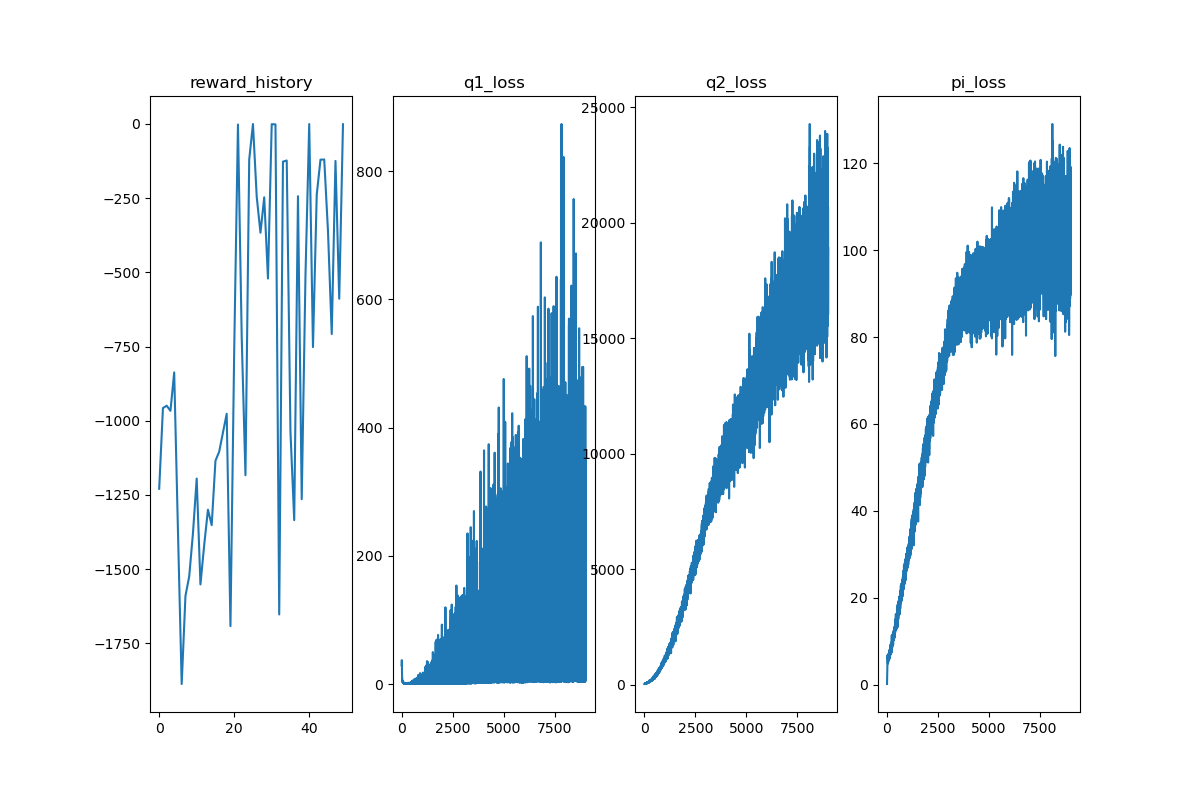
\includegraphics[width=0.45\textwidth]{sac-pendulum}
    \caption{SAC in the Pendulum-v1 Environment}
\end{figure}

\blindtext

\subsection{Ant-v3}

\begin{figure}
    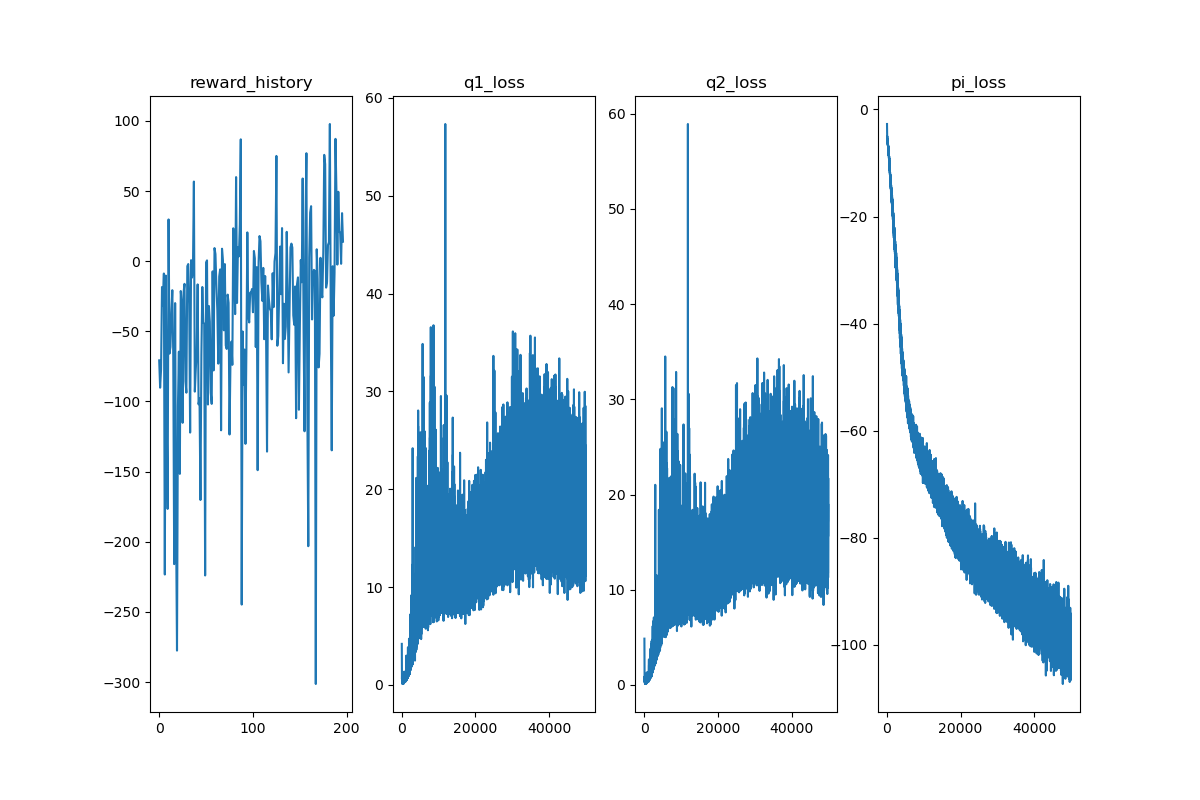
\includegraphics[width=0.45\textwidth, height=5cm]{sac-ant}
    \caption{SAC in the Ant-v3 environment}
\end{figure}

\begin{figure}
    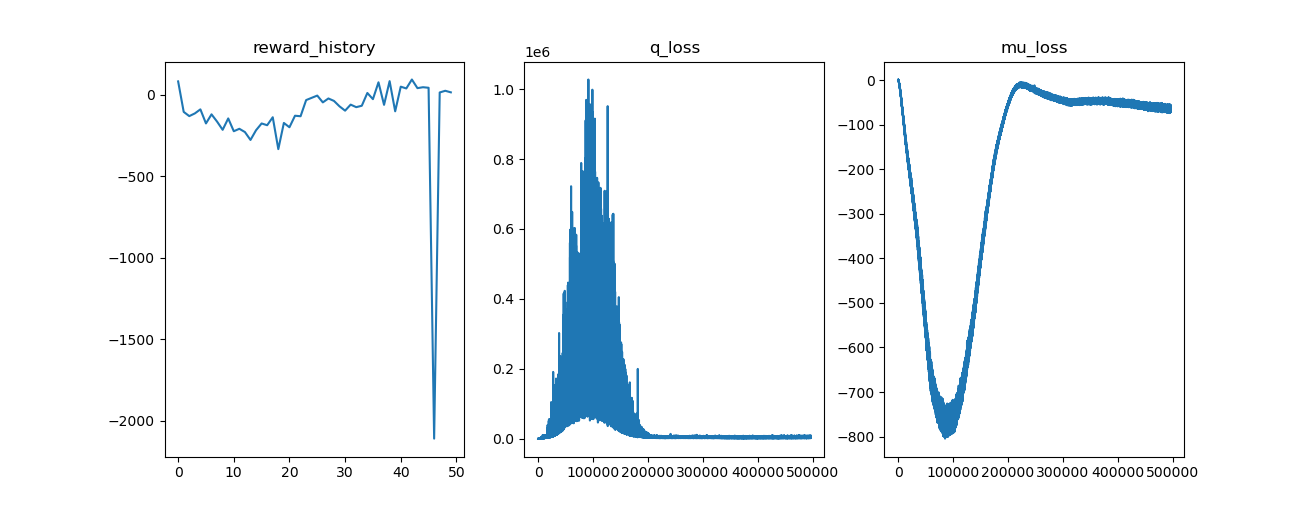
\includegraphics[width=0.45\textwidth, height=5cm]{ddpg-ant}
    \caption{DDPG in the Ant-v3 environment}
\end{figure}

\blindtext

\subsection{Humanoid-v3}

\blindtext

\section{Future Work and Conclusions}

\blindtext[2]


\bibliography{references}
\bibliographystyle{ieeetran}


\end{document}
